For robustness, we use nearest propensity score matching to match each zipcode from treatment group with an equivalent control group, using zip code level demographics. After matching, we have left with 89 matched zip codes. Below are the propensity score before and after matching.

\begin{figure}
     \centering
     \begin{subfigure}
         \centering
         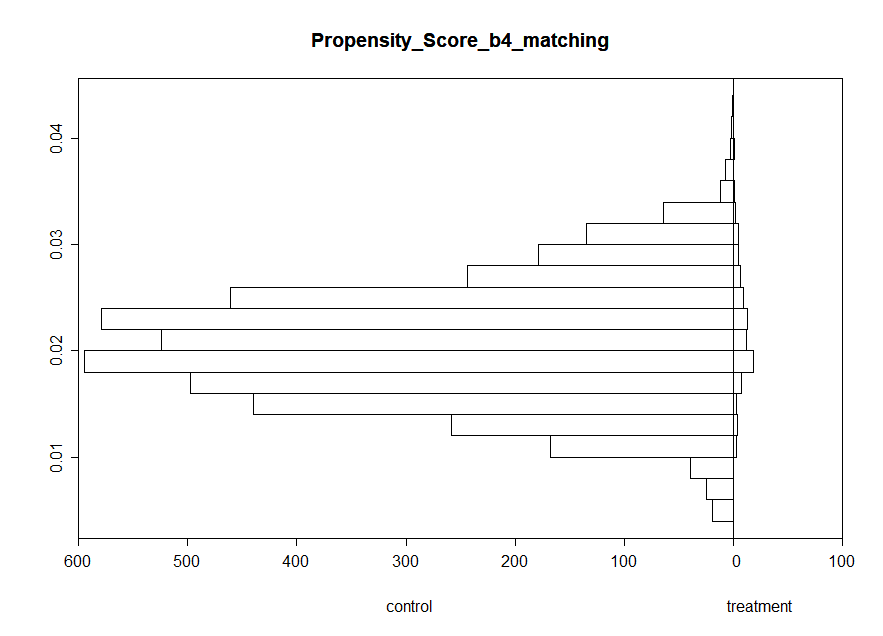
\includegraphics[width=\textwidth]{b4matching.png}
         \label{fig:b4matching}
     \end{subfigure}
     \hfill
     \begin{subfigure}
         \centering
         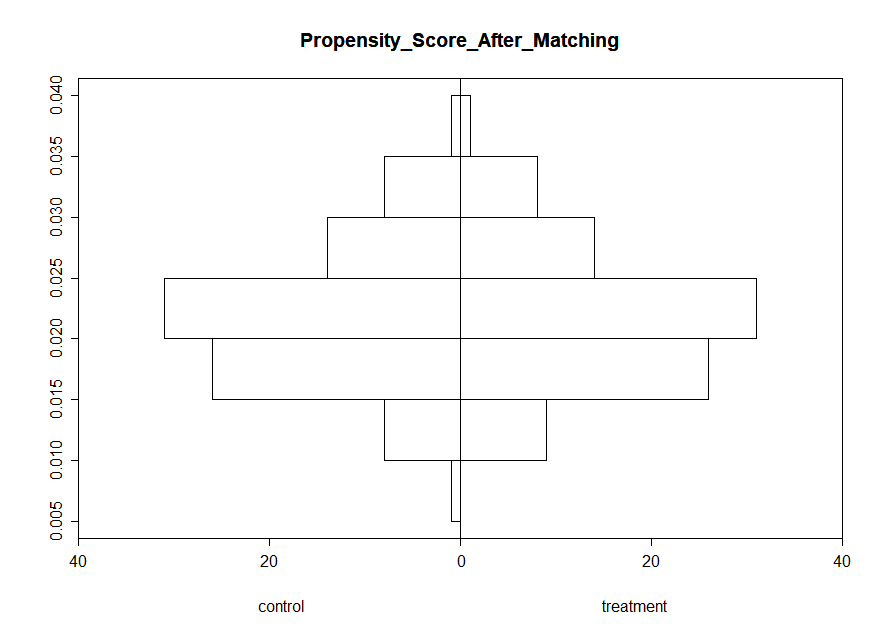
\includegraphics[width=\textwidth]{Aftermatching.png}
         \label{fig:aftermatching}
     \end{subfigure}
\end{figure}

\begin{table}[!htbp] \centering 
      \caption{Results of the Online Sales and Search Effect After Nearest Propensity Score Matching: TotalMonthlySales, PagesPerDollar, and MinsPerDollar (All Product Categories)} 
      \label{tab:tablepsm} 
      \resizebox{\columnwidth}{!}{
            \begin{tabular}{@{\extracolsep{1pt}}lD{.}{.}{-3} D{.}{.}{-3} D{.}{.}{-3} D{.}{.}{-3} D{.}{.}{-3} D{.}{.}{-3} } 
             \\[-1.8ex]\hline 
             \hline \\[-1.8ex] 
              % & \multicolumn{6}{c}{\textit{Dependent variable:}} \\ 
              %\cline{2-7} 
              %\\[-1.8ex]
              & \multicolumn{2}{c}{log(TotalMonthlySales + 1)} & \multicolumn{2}{c}{log(PagesPerDollar + 1)} & \multicolumn{2}{c}{log(MinsPerDollar + 1)} \\ 
              & \multicolumn{1}{c}{Amazon-0 Mile} & \multicolumn{1}{c}{BesyBuy-0 Mile} & \multicolumn{1}{c}{Amazon-0 Mile} & \multicolumn{1}{c}{BesyBuy-0 Mile} &                             \multicolumn{1}{c}{Amazon-0 Mile} & \multicolumn{1}{c}{BesyBuy-0 Mile} \\ 
              \\[-1.8ex] & \multicolumn{1}{c}{(1)} & \multicolumn{1}{c}{(2)} & \multicolumn{1}{c}{(3)} & \multicolumn{1}{c}{(4)} & \multicolumn{1}{c}{(5)} & \multicolumn{1}{c}               {(6)}\\ 
              \hline \\[-1.8ex] 
              $beta_1$ & 0.029 & 0.0002 & 0.00004 & 0.0001 & 0.002 & 0.00000 \\ 
               & (0.024) & (0.031) & (0.020) & (0.009) & (0.019) & (0.005) \\ 
              $beta_2$ & -0.033 & 0.009 & -0.068^{***} & 0.003 & -0.057^{***} & 0.0004 \\ 
              & (0.028) & (0.031) & (0.023) & (0.009) & (0.022) & (0.005) \\ 
              \hline \\[-1.8ex] 
              Observations & \multicolumn{1}{c}{3,000} & \multicolumn{1}{c}{768} & \multicolumn{1}{c}{3,000} & \multicolumn{1}{c}{768} & \multicolumn{1}{c}{3,000} &                           \multicolumn{1}{c}{768} \\ 
              R$^{2}$ & \multicolumn{1}{c}{0.001} & \multicolumn{1}{c}{0.001} & \multicolumn{1}{c}{0.004} & \multicolumn{1}{c}{0.001} & \multicolumn{1}{c}{0.003} &                           \multicolumn{1}{c}{0.00004} \\ 
              Adjusted R$^{2}$ & \multicolumn{1}{c}{-0.052} & \multicolumn{1}{c}{-0.078} & \multicolumn{1}{c}{-0.048} & \multicolumn{1}{c}{-0.078} & \multicolumn{1}{c}{-0.049}               & \multicolumn{1}{c}{-0.079} \\ 
              F Statistic & \multicolumn{1}{c}{0.935 (df = 2; 2850)} & \multicolumn{1}{c}{0.192 (df = 2; 711)} & \multicolumn{1}{c}{6.219$^{***}$ (df = 2; 2850)} &                           \multicolumn{1}{c}{0.185 (df = 2; 711)} & \multicolumn{1}{c}{4.693$^{***}$ (df = 2; 2850)} & \multicolumn{1}{c}{0.014 (df = 2; 711)} \\ 
              \hline 
              \hline \\[-1.8ex] 
              \textit{Note:}  & \multicolumn{6}{r}{$^{*}$p$<$0.1; $^{**}$p$<$0.05; $^{***}$p$<$0.01} \\ 
              \end{tabular}}
\end{table}

The code for generating Table \ref{tab:tablepsm} are listed as below.
\lstinputlisting[language=R, caption={Table PSM Generation}, label={lst:tablepsm}, linerange={138-172, 216-237}]{../psm.R}
